\chapter{Randomness}
\label{Statistical Tests for Randomness}
\minitoc

\section{Some famous statistical tests of random number generators}
\label{Some famous statistical tests of random number generators}

A theoretical proof for the randomness of a generator is impossible to give, therefore statistical inference based on observed sample sequences produced by the generator seems to be the best option. Considering the properties of binary
random sequences, various statistical tests can be designed to evaluate the assertion
that the sequence is generated by a perfectly random source. 
We have performed certain statistical tests for various CI PRNGs we proposed. These tests
include TestU01~\cite{Lecuyer2009}, NIST suite~\cite{ANDREW2008},
Diehard battery of tests~\cite{Marsaglia1996}, and Comparative test parameters. For completeness and for reference, we give
in the following subsection a brief description of each of the
aforementioned tests.



\subsection{NIST statistical test suite}



Among the numerous standard tests for pseudo-randomness, a convincing way to show the randomness of the produced sequences is to confront them to the NIST (National Institute of  Standards and Technology) Statistical Test, because it is an up-to-date test suite proposed by the Information Technology Laboratory (ITL). A new version of the Statistical Test Suite (Version 2.0) has been released in August 11, 2010.


The NIST test suite SP 800-22 is a statistical package consisting of 15 tests. They were developed to test the randomness of binary sequences produced by hardware or software based cryptographic PRNGs. These tests focus on a variety of different types of non-randomness that could exist in a sequence. 


For each statistical test, a set of $P-values$ (corresponding to the set of sequences) is produced. The interpretation of empirical results can be conducted in any number of ways. In this paper, the examination of the distribution of P-values to check for uniformity ($ P-value_{T}$) is used.
The distribution of P-values is examined to ensure uniformity. 
If $P-value_{T} \geqslant 0.0001$, then the sequences can be considered to be uniformly distributed.

In our experiments, 100 sequences (s = 100), each with 1,000,000-bit long, are generated and tested. If the $P-value_{T}$ of any test is smaller than 0.0001, the sequences are considered to be not good enough and the generating algorithm is not suitable for usage.

In what follows, the fifteen tests of the NIST Statistical tests suite, are recalled. A more detailed description for those tests could be found in \cite{ANDREW2008}.
\begin{itemize}
\item \textbf{Frequency (Monobit) Test (FT)} is to determine whether the number of ones and zeros in a sequence are approximately the same as would be expected for a truly random sequence.


\item \textbf{Frequency Test within a Block (FBT)} is to determine whether the frequency of ones in an M-bit block is approximately $M/2$, as would be expected under an assumption of randomness.($M$ is the length of each block.)


\item \textbf{Runs Test (RT)} is to determine whether the number of runs of ones and zeros of various lengths is as expected for a random sequence. In particular, this test determines whether the oscillation between such zeros and ones is too fast or too slow.


\item \textbf{Test for the Longest Run of Ones in a Block (LROBT)} is to determine whether the length of the longest run of ones within the tested sequence is consistent with the length of the longest run of ones that would be expected in a random sequence.


\item \textbf{Binary Matrix Rank Test (BMRT)} is to check for linear dependence among fixed length substrings of the original sequence.


\item \textbf{Discrete Fourier Transform (Spectral) Test (DFTT)} is to detect periodic features (i.e., repetitive patterns that are near each other) in the tested sequence that would indicate a deviation from the assumption of randomness.


\item \textbf{Non-overlapping Template Matching Test (NOTMT)} is to detect generators that produce too many occurrences of a given non-periodic (aperiodic) pattern.(m is the length in bits of each template which is the target string.)


\item \textbf{Overlapping Template Matching Test (OTMT)} is the number of occurrences of pre-specified target strings.(m is the length in bits of the template--in this case, the length of the run of ones.)

\item \textbf{Maurer's ``Universal Statistical`` Test (MUST)} is to detect whether or not the sequence can be
significantly compressed without loss of information.(L is the length of each block, and Q is the number of blocks in the initialization sequence)

\item \textbf{Linear Complexity Test (LCT)} is to determine whether or not the sequence is complex enough to be considered random.(M is the length in bits of a block.)

\item \textbf{Serial Test (ST)} is to determine whether the number of occurrences of the $2^{m}$ m-bit.(m is the length in bits of each block.)
overlapping patterns is approximately the same as would be expected for a random sequence.

\item \textbf{Approximate Entropy Test (AET)} is to compare the frequency of overlapping blocks of two consecutive/adjacent lengths (m and m+1) against the expected result for a random sequence.(m is the length of each block.)

\item \textbf{Cumulative Sums (Cusum) Test (CST)} is to determine whether the cumulative sum of the partial sequences occurring in the tested sequence is too large or too small relative to the expected behavior of that cumulative sum for random sequences.

\item \textbf{Random Excursions Test (RET)} is to determine if the number of visits to a particular state within a cycle deviates from what one would expect for a random
sequence.

\item \textbf{Random Excursions Variant Test (REVT)} is to detect deviations from the expected number
of visits to various states in the random walk.
\end{itemize}

\subsection{Diehard battery of tests}
The Diehard battery of tests was developed in 1996 by Prof. Georges Marsaglia
from the Florida State University for testing randomness of sequences of numbers
[77]. 
It has been the most sophisticated standard for over a decade. Because of the stringent requirements in the Diehard test suite, a generator passing Diehard battery of 
tests can be considered good as a rule of thumb. It was supposed to give a better way of analysis in comparison to original FIPS statistical tests.

The Diehard battery of tests consists of 18 different independent statistical tests. 
Each test requires binary file of about 10-12 million bytes in order to run the full set of tests. 
As the NIST test suite, most of the tests in Diehard return a $p-value$, which should be uniform on $[0,1)$ if the input file 
contains truly independent random bits.  Those $p-value$s are obtained by                
$p=F(X)$, where $F$ is the assumed distribution of the sample random variable $X$ (often normal). 
But that assumed $F$ is just an asymptotic approximation, for which the fit will be worst             
in the tails. Thus occasional $p-value$s near 0 or 1, such as 0.0012 or 0.9983 can occur. Unlike the NIST test suite, the test is considered to be successful when
the $p-value$ is in range where $[0 + \alpha , 1 -\alpha ]$ is the level of significance of the test.                
  
For example, with a level of significance of $5\%$, p-value are expected to be in
$[0.025, 0.975]$. Note that if the $p-value$ is not in this range, it means that the null
hypothesis for randomness is rejected even if the sequence is truly random. These
tests are:
\begin{itemize}
\item \textbf{Birthday Spacings} Choose random points on a large interval. The spacings
between the points should be asymptotically Poisson distributed. The name
is based on the birthday paradox.
\item \textbf{Overlapping Permutations} Analyze sequences of five consecutive random
numbers. The 120 possible orderings should occur with statistically equal
probability
\item \textbf{Ranks of matrices} Select some number
of bits from some number of random numbers to form a matrix over 0,1, then
determine the rank of the matrix. Count the ranks.
\item \textbf{Monkey Tests} Treat sequences of some number of bits as ''words''. Count
the overlapping words in a stream. The number of ''words'' that don't appear
should follow a known distribution. The name is based on the infinite monkey
theorem.
\item \textbf{Count the 1's} Count the 1 bits in each of either successive
or chosen bytes. Convert the counts to ''letters'', and count the occurrences
of five-letter ''words''
\item \textbf{Parking Lot Test} Randomly place unit circles in a $100 x 100 $square. If the
circle overlaps an existing one, try again. After 12,000 tries, the number of
successfully ''parked'' circles should follow a certain normal distribution.
\item \textbf{Minimum Distance Test} Randomly place 8,000 points in a $10,000 x 10,000$
square, then find the minimum distance between the pairs. The square of this
distance should be exponentially distributed with a certain mean.
\item \textbf{Random Spheres Test} Randomly choose 4,000 points in a cube of edge 1,000.
Center a sphere on each point, whose radius is the minimum distance to another point. The smallest sphere's volume should be exponentially distributed
with a certain mean.
\item \textbf{The Sqeeze Test} Multiply 231 by random floats on [0,1) until you reach 1.
Repeat this 100,000 times. The number of floats needed to reach 1 should
follow a certain distribution.
\item \textbf{Overlapping Sums Test} Generate a long sequence of random floats on [0,1).
Add sequences of 100 consecutive floats. The sums should be normally distributed with characteristic mean and sigma.
\item \textbf{Runs Test} Generate a long sequence of random floats on [0,1). Count ascending and descending runs. The counts should follow a certain distribution.
\item \textbf{The Craps Test} Play 200,000 games of craps, counting the wins and the number
of throws per game. Each count should follow a certain distribution.
\end{itemize}



\subsection{Comparative test parameters}

In this section, five well-known statistical tests~\cite{Menezes1997} are used as  comparison tools. They encompass frequency and autocorrelation tests. In what follows, $s = s^0,s^1,s^2,\dots , s^{n-1}$ denotes a binary sequence of length $n$. The question is to determine whether this sequence possesses some specific characteristics that a truly random sequence would be likely to exhibit. The tests are introduced in this subsection and results are given in the next one.

\paragraph{Frequency test (monobit test)}

The purpose of this test is to check if the numbers of 0's and 1's are approximately equal in $s$, as it would be expected for a random sequence. Let $n_0, n_1$ denote these numbers. The statistic used here is 
\begin{equation*}
X_1=\frac{(n_0-n_1)^2}{n}, 
\end{equation*}
which approximately follows a $\chi^2$ distribution with one degree of freedom when $n\geqslant 10^7$.

\paragraph{Serial test (2-bit test)}

The purpose of this test is to determine if the number of occurrences of 00, 01, 10 and 11 as subsequences of $s$ are approximately the same. Let $n_{00} , n_{01} ,n_{10}$, and $n_{11}$ denote the number of occurrences of $00, 01, 10$, and $11$ respectively. Note that $n_{00} + n_{01} + n_{10} + n_{11} = n-1$ since the subsequences are allowed to overlap. The
statistic used here is:
\begin{equation*}
X_2=\frac{4}{n-1}(n_{00}^2+n_{01}^2+n_{10}^2+n_{11}^2)-\frac{2}{n}(n_0^2+n_1^2)+1,
\end{equation*}
 which approximately follows a $\chi^2$ distribution with 2 degrees of freedom if $n\geqslant 21$.

\paragraph{Poker test}

The poker test studies if each pattern of length $m$ (without overlapping) appears the same number of times in $s$. Let $\lfloor \frac{n}{m} \rfloor\geqslant 5 \times 2^m$ and $k= \lfloor \frac{n}{m} \rfloor $. Divide the sequence $s$ into $k$ non-overlapping parts, each of length $m$. Let $n_i$ be the number of occurrences of the $i^{th}$ type of sequence of length $m$, where $1 \leqslant i \leqslant 2^m$. The statistic used is 
\begin{equation*}
X_3=\dfrac{2^m}{k}\left(\displaystyle{\sum^{2^m}_{i=1}n^2_i}\right)-k,
\end{equation*}
which approximately follows a $\chi^2$ distribution with $2^m-1$ degrees of freedom. Note that the poker test is a generalization of the frequency test (setting $m = 1$ in the poker test yields the frequency test).

\paragraph{Runs test}

The purpose of the runs test is to figure out whether the number of runs of various lengths in the sequence $s$ is as expected, for a random sequence. A run is defined as a pattern of all zeros or all ones, a block is a run of ones, and a gap is a run of zeros. The expected number of gaps (or blocks) of length $i$ in a random sequence of length $n$ is $e_i = \frac{n-i+3}{2^{i+2}}$. Let $k$ be equal to the largest integer $i$ such that $e_i \geqslant 5$. Let
$B_i , G_i$ be the number of blocks and gaps of length $i$ in $s$, for each $i \in \llbracket 1, k\rrbracket$. The statistic used here will then be:
\begin{equation*}
\displaystyle{X_4=\sum^k_{i=1}\frac{(B_i-e_i)^2}{e_i}+\sum^k_{i=1}\frac{(G_i-e_i)^2}{e_i}},
\end{equation*}
\noindent which approximately follows a $\chi^2$ distribution with $2k - 2$ degrees of freedom.

\paragraph{Autocorrelation test}

The purpose of this test is to check for coincidences between the sequence $s$ and (non-cyclic) shifted versions of it. Let $d$ be a fixed integer, $ 1 \leqslant d \leqslant \lfloor n/2 \rfloor$. The  $A(d) = \sum_{i=0}^{n-d-1} s_i\oplus s_{i+d}$ is the amount of bits not equal between the sequence and itself displaced by $d$ bits. The statistic used is:
\begin{equation*}
X_5=\dfrac{2 \left(A(d)-\frac{n-d}{2}\right)}{\sqrt{n-d}},
\end{equation*}
which approximately follows a normal distribution $\mathcal{N}(0, 1)$ if $n-d \geqslant 10$. Since small values of $A(d)$ are as unexpected as large values, a two-sided test should be used.

\subsection{TestU01 Statistical Test}
\label{Testing a generator}

TestU01 is extremely diverse in implementing classical tests,
cryptographic tests, new tests proposed in the literature, and original tests.
In fact, it encompasses most of the other testsuites. 
Seven batteries of tests in the TestU01 package are listed as follows:

\begin{itemize}
\item{\textbf{Small Crush.}} The first battery to check, with 15 $p-$values reported. This is a fast collection of tests used to be sure that the basic requirements of randomness are satisfied. In case of success, this battery should be followed by Crush and BigCrush.
\item{\textbf{Crush.}} This battery includes many difficult tests, like those described in ~\cite{Knuth1998}. %Cette référence n'apparaît pas.
%D. E. Knuth. The Art of Computer Programming, Volume 2: Seminumerical Algorithms. Addison-Wesley, Reading, Mass., third edition, 1998.
It uses approximately $2^35$ random numbers and applies 96 statistical tests
(it computes a total of 144 test statistics and p-values)
\item{\textbf{Big Crush.}} it uses
approximately $2^38$ random numbers and applies 106 tests (it computes 160 test
statistics and p-values)
A suite of very stringent statistical tests, and the most difficult battery to pass.
\item{\textbf{Rabbit.}} This battery of tests reports 38 $p-$values.
\item{\textbf{Alphabit.}} Alphabit and AlphabitFile have been designed primarily to test hardware random bits generators. 17 $p-$values are reported.
\item{\textbf{Pseudo-DieHARD.}} This battery implements most of the tests contained in the popular battery DieHARD or, in some cases, close approximations to them. It is not a very stringent battery. Indeed, there is no generator that can pass Crush and BigCrush batteries and fail Pseudo-DieHARD, while the converse occurs for several defective generators. 126 $p-$values are reported here.
\item{\textbf{FIPS\_140\_2.}} The NIST (National Institute of Standards and Technology) of the U.S. federal government has proposed a statistical test suite. It is used to evaluate the randomness of bitstreams produced by cryptographic random number generators. This battery reports 16 $p-$values.
\end{itemize}

Six predefined batteries of tests are available in TestU01; three of them
are for sequences of U (0, 1) random numbers and the three others are for bit
sequences. In the first category, we have SmallCrush, Crush, and BigCrush
To test a RNG for general use.
one could first apply the small and fast battery SmallCrush. If it passes, one could then apply
the more stringent battery Crush, and finally the yet more time-consuming battery BigCrush.
These batteries of tests include the classical tests described in Knuth~\cite{Knuth1998}, for
example, the run, poker, coupon collector, gap, max-of-t, and permutation tests.
There are collision and birthday spacings tests in 2, 3, 4, 7, 8 dimensions, several close pairs tests in 2, 3, 5, 7, 9 dimensions, and correlation tests. Some
tests use the generated numbers as a sequence of ``random`` bits: random walk
tests, linear complexity tests, a Lempel-Ziv compression test, several Hamming
weights tests, matrix rank tests, run and correlation tests, among others.




The batteries Rabbit, Alphabit, and BlockAlphabit are for binary sequences
(e.g., a cryptographic pseudorandom generator or a source of random bits
produced by a physical device). They were originally designed to test a finite
sequence contained in a binary file. When invoking the battery, one must specify the number $n_B$ of bits available for each test. When the bits are in a file, $n_B$
must not exceed the number of bits in the file, and each test will reuse the same
sequence of bits starting from the beginning of the file (so the tests are not independent). When the bits are produced by a generator, each test uses a different
stream. In both cases, the parameters of each test are chosen automatically as
a function of $n_B$ .
The batteries Alphabit and Rabbit can be applied on a binary file considered as a source
of random bits. They can also be applied on a programmed generator. Alphabit has been
defined primarily to test hardware random bits generators. The battery PseudoDIEHARD
applies most of the tests in the well-known DIEHARD suite of Marsaglia [106]. The battery
FIPS\_140\_2 implements the small suite of tests of the FIPS\_140\_2 standard from NIST.
The batteries described in this module will write the results of each test (on standard
output) with a standard level of details (assuming that the boolean switches of module
swrite have their default values), followed by a summary report of the suspect p-values
obtained from the specific tests included in the batteries. It is also possible to get only the
summary report in the output, with no detailed output from the tests, by setting the boolean
switch swrite\_Basic to FALSE. Rabbit and Alphabit apply 38 and 17 different statistical tests,
respectively. 

Some of the tests compute more than one statistic (and p-value) using the same stream of random
numbers and these statistics are thus not independent. That is why the number of statistics
in the summary reports is larger than the number of tests in the description of the batteries.


\begin{itemize}
\item{\textbf{Small Crush.}}  smarsa\_BirthdaySpacings   \\ 
 sknuth\_Collision   \\ 
 sknuth\_Gap    \\ 
 sknuth\_SimpPoker   \\ 
 sknuth\_CouponCollector    \\ 
 sknuth\_MaxOft   \\ 
 svaria\_WeightDistrib     \\ 
 smarsa\_MatrixRank     \\  
 sstring\_HammingIndep    \\ 
 swalk\_RandomWalk1      \\ 
\item{\textbf{Crush.}}  smarsa\_SerialOver   \\    
 smarsa\_CollisionOver      \\ 
 smarsa\_BirthdaySpacings      \\ 
 snpair\_ClosePairs      \\ 
 snpair\_ClosePairsBitMatch     \\  
 sknuth\_SimpPoker      \\ 
 sknuth\_CouponCollector      \\ 
 sknuth\_Gap      \\ 
 sknuth\_Run      \\ 
 sknuth\_Permutation      \\ 
 sknuth\_CollisionPermut      \\ 
 sknuth\_MaxOft      \\ 
 svaria\_SampleProd      \\ 
 svaria\_SampleMean     \\ 
 svaria\_SampleCorr      \\ 
 svaria\_AppearanceSpacings   \\    
 svaria\_WeightDistrib     \\  
 svaria\_SumCollector      \\ 
 smarsa\_MatrixRank      \\ 
 smarsa\_Savir2      \\ 
 smarsa\_GCD      \\ 
 swalk\_RandomWalk1      \\ 
 scomp\_LinearComp     \\  
 scomp\_LempelZiv      \\ 
 sspectral\_Fourier3      \\ 
 sstring\_LongestHeadRun     \\  
 sstring\_PeriodsInStrings    \\   
 sstring\_HammingWeight2      \\ 
 sstring\_HammingCorr      \\ 
 sstring\_HammingIndep     \\  
 sstring\_Run      \\ 
 sstring\_AutoCor   \\ 
\item{\textbf{Big Crush.}} smarsa\_SerialOver\\ 
smarsa\_CollisionOver\\ 
smarsa\_BirthdaySpacings\\ 
snpair\_ClosePairs \\ 
sknuth\_SimpPoker\\ 
sknuth\_CouponCollector\\ 
sknuth\_Gap\\ 
sknuth\_Run\\ 
sknuth\_Permutation\\ 
sknuth\_CollisionPermut\\ 
sknuth\_MaxOft\\ 
svaria\_SampleProd\\ 
svaria\_SampleMean\\ 
svaria\_SampleCorr\\ 
svaria\_AppearanceSpacings\\ 
svaria\_WeightDistrib\\ 
svaria\_SumCollector\\ 
smarsa\_MatrixRank\\ 
smarsa\_Savir2\\ 
smarsa\_GCD\\ 
swalk\_RandomWalk1\\ 
scomp\_LinearComp\\ 
scomp\_LempelZiv\\ 
sspectral\_Fourier3\\ 
sstring\_LongestHeadRun\\ 
sstring\_PeriodsInStrings\\ 
sstring\_HammingWeight2\\ 
sstring\_HammingCorr\\ 
sstring\_HammingIndep\\ 
sstring\_Run\\ 
sstring\_AutoCor\\ 

\item{\textbf{Rabbit.}} smultin\_MultinomialBitsOver\\ 
snpair\_ClosePairsBitMatch\\ 
svaria\_AppearanceSpacings\\ 
scomp\_LinearComp\\ 
scomp\_LempelZiv\\ 
sspectral\_Fourier1\\ 
sspectral\_Fourier3\\ 
sstring\_LongestHeadRun\\ 
sstring\_PeriodsInStrings\\ 
sstring\_HammingWeight\\ 
sstring\_HammingCorr\\ 
sstring\_HammingIndep\\ 
sstring\_AutoCor\\ 
sstring\_Run\\ 
smarsa\_MatrixRank\\ 
swalk\_RandomWalk1\\ 

\item{\textbf{Alphabit.}} smultin\_MultinomialBitsOver\\ 
sstring\_HammingIndep\\ 
sstring\_HammingCorr\\ 
swalk\_RandomWalk1 \\ 


\item{\textbf{Pseudo-DieHARD.}} Birthday Spacings test\\ 
Overlapping 5-Permutation test\\ 
Binary Rank Tests for Matrices test\\ 
Bitstream test\\ 
OPSO test\\ 
OQSO test\\ 
DNA test\\ 
Count-the-1's test\\ 
Parking Lot test\\ 
Minimum Distance test\\ 
3-D Spheres test\\ 
Squeeze test\\ 
Overlapping Sums test\\ 
Runs test\\ 
Craps test\\ 

\item{\textbf{FIPS\_140\_2.}} Monobit test\\ 
``poker'' test\\ 
Runs test\\ 
Longest Run of Ones in a Block test

\end{itemize}

TestU01 suite implements hundreds of tests and reports $p-$values. If a $p-$value is within $[0.001,0.999]$, the associated test is a success. A $p-$value lying outside this boundary means that its test has failed. %This is the standard range the test-suite suggests. The p-value selection criteria for the various test suites were chosen to produce a few failures in the best cases. Setting the criteria too low (closer to zero) would exhibit no failures and setting the criteria too high would fail everything.



\section{Test results for some PRNGs}

\subsection{Results of NIST}

In our experiments, 100 sequences (s = 100) of 1,000,000 bits are generated and tested. If the value $\mathbb{P}_T$ of any test is smaller than 0.0001, the sequences are considered to not be good enough and the generator is unsuitable. Table~\ref{The passing1} shows $\mathbb{P}_T$ of the sequences for Logistic map, XORshift and ISAAC in Section~\ref{The generation of pseudorandom sequence}. If there are at least two statistical values in a test, this test is marked with an asterisk and the average value is computed to characterize the statistical values. 


\begin{table}[!t]
\renewcommand{\arraystretch}{1.3}
\caption{NIST SP 800-22 test results ($\mathbb{P}_T$)}
\label{The passing1}
\centering
  \begin{tabular}{lccc}
    \toprule
Test name &Logistic& XORshift& ISAAC\\ 

Frequency (Monobit) Test 					&0.53414		&0.14532		&0.67868 \\ 
Frequency Test within a Block  					&0.00275		&0.45593		&0.10252 \\ 
Runs Test 							&0.00001		&0.21330		&0.69931  \\ 
Longest Run of Ones in a Block Test 				&0.08051		&0.28966		&0.43727   \\
Binary Matrix Rank Test 					&0.67868		&0.00000		&0.89776  \\ 
Discrete Fourier Transform (Spectral) Test			&0.57490		&0.00535		&0.51412   \\ 
Non-overlapping Template Matching Test* 			&0.28468		&0.50365		&0.55515  \\ 
Overlapping Template Matching Test   				&0.10879		&0.86769		&0.63711  \\ 
Universal Statistical Test   					&0.02054		&0.27570		&0.69931   \\ 
Linear Complexity Test  					&0.79813		&0.92407		&0.03756    \\ 
Serial Test* (m=10) 						&0.41542		&0.75792		&0.32681   \\ 
Approximate Entropy Test (m=10) 				&0.02054		&0.41902		&0.30412  \\ 
Cumulative Sums (Cusum) Test* 					&0.60617		&0.81154		&0.36786\\ 
Random Excursions Test* 					&0.53342		&0.41923		&0.50711   \\ 
Random Excursions Variant Test* 				&0.28507		&0.52833		&0.40930    \\ \hline
Success 							&15/15		&14/15			&15/15 \\ 
\bottomrule
  \end{tabular}
\end{table}

\subsection{Results of Diehard}
\label{Subsec:DieHARD}

Table~\ref{Results of DieHARD battery} gives the results derived from applying the DieHARD battery of tests to Logistic map, XORshift and ISAAC in Section~\ref{The generation of pseudorandom sequence}.

\begin{tiny}
\begin{table}[!t]
\renewcommand{\arraystretch}{1.3}
\caption{Results of DieHARD battery of tests}
\label{Results of DieHARD battery}
\centering
\begin{tabular}{llccc} \toprule
No. &Test name &Logistic& XORshift& ISAAC\\
1 & Overlapping Sum  &Pass &Pass&Pass\\
2 & Runs Up 1  & Pass &Pass&Pass\\
&Runs Down 1  &Pass &Pass&Pass\\
&Runs Up 2  &Pass &Pass&Pass\\
&Runs Down 2  & Pass &Pass&Pass\\
3 & 3D Spheres  &Pass &Pass&Pass\\
4 & Parking Lot  &Pass &Pass&Pass\\
5 & Birthday Spacing  &Pass &Pass&Pass\\
6 & Count the ones 1  &Pass &Fail&Pass\\
7 &Binary Rank $6 \times 8$  & Pass &Pass&Pass\\
8 &Binary Rank $31 \times 31$  &Pass &Fail&Pass\\
9 &Binary Rank $32 \times 32$  &Pass &Fail&Pass\\
10 &Count the ones 2  &Pass&Pass&Pass \\
11 &Bit Stream  &Pass&Pass&Pass \\
12 &Craps Wins  &Pass&Pass&Pass \\
&Throws &Pass  &Pass&Pass\\
13 &Minimum Distance  &Pass &Pass&Pass\\
14 &Overlapping Perm.  &Pass &Pass&Pass\\
15 &Squeeze &Pass &Pass&Pass \\
16 &OPSO &Pass &Pass&Pass \\
17 &OQSO &Pass &Pass&Pass \\
18 &DNA &Pass &Pass &Pass\\
&Number of tests passed  &18 &15&18\\\bottomrule
\end{tabular}
\end{table}
\end{tiny}

\subsection{Results of comparative test parameters}



\begin{table}[!t]
\renewcommand{\arraystretch}{1.3}
\caption{Comparative test parameters with a $10^7$ bits sequence}
\label{Comparison3}
\centering
  \begin{tabular}{lcccc}
   \toprule
Method			&Threshold values 	 		&Logistic	& XORshift	& ISAAC\\
Monobit			&3.8415					&0.1280		&1.7053		&0.1401\\ \hline
Serial  		&5.9915 				&0.1302		&2.1466		&0.1430  \\ \hline
Poker  			&316.9194 				&240.2893	&248.9318	&236.8670  \\ \hline
Runs 			&55.0027				&26.5667	&18.0087	&34.1273   \\ \hline
Autocorrelation		&1.6449			 		& 0.0373	&0.5099 	&-2.1712  \\ 
\bottomrule
  \end{tabular}
\end{table}

We show in Table~\ref{Comparison3} a comparison between Logistic map, XORshift and ISAAC in Section~\ref{The generation of pseudorandom sequence}. 



\subsection{Results of TestU01}

Table~\ref{TestU011} gives the results derived from applying the TestU01 battery of tests to the PRNGs considered in Logistic map, XORshift and ISAAC in Section~\ref{The generation of pseudorandom sequence}.
\begin{table}[!t]
\renewcommand{\arraystretch}{1.3}
\caption{TestU01 Statistical Test}
\label{TestU011}
\centering
  \begin{tabular}{lcccccc}
    \toprule
Test name &Battery&Parameters& Logistic 		& XORshift	& ISAAC\\
Rabbit 				&$32\times10^9$ bits  	&38	&21  	 	&14	&0	 \\
Alphabit 			&$32\times10^9$ bits	&17	&16 		&9	&0	 \\
Pseudo DieHARD 			&Standard		&126	&0 	 	&2	&0	\\
FIPS\_140\_2 			&Standard		&16	&0 		&0	&0	\\
Small Crush 			&Standard		&15	&4 		&5	&0	 \\
Crush 				&Standard		&144	&95 		&57	&0	 \\
Big Crush 			&Standard		&160	&125 	 	&55	&0	 \\ \hline
Number of failures 		& 			&516	&261 	 	&146	&0	 \\
\bottomrule
  \end{tabular}
\end{table}



\subsection{Conclusion}
From the results of the TestU01, NIST, Comparative test parameters and DieHARD batteries of tests applied to Logistic map, XORshift and ISAAC in Section~\ref{The generation of pseudorandom sequence}, the worst situation obviously appears when using the logistic map or XORshift, and  ISAAC can pass the three batteries of tests.

We can conclude that Binary Matrix Rank Test is failed for XORshift in NIST statistical test suite. The focus of the test is the rank of disjoint sub-matrices of the entire sequence. Note that this test also appears in the DIEHARD battery of tests.

XORshift fails three individual tests contained into the DieHARD battery, namely: ``Count the ones'', ``Binary Rank $31 \times 31$'', and ``Binary Rank $32 \times 32$''. 
We can thus conclude that, in the random numbers obtained with XORshift, only the least significant bits seem to be independent. This fact can explain the poor behavior of this PRNG in the aforementioned basic tests that evaluate the independence of real numbers. 


Seven tests were failed with a $p-value$ practically equal to 0 or 1 for logistic map and XORshift in TestU01 Statistical Test. It is clear that the null hypothesis $H_0$ must be rejected for these two bit streams. $H_0$ is equivalent to saying that for each integer $t>0$, the vector $(u_0 , . . . , u_{t-1} ) $is uniformly distributed over the $t$-dimensional unit cube $[0, 1]^t$



\section{Test results and comparative analysis for old CI}
\label{Test results and comparative analysis}

\subsection{How to choose good parameters}

\subsubsection{Small Crush test and correlation with $k$}

To exhibit the correlation between the parameter $k$ such that $\mathcal{M}=\{$k, k+1$\}$ (see Section \ref{subsec Chaotic iterations as PRNG}) and the success rate, we have used CI(ISAAC, XORshift) PRNG as a concrete example. 

%We are now ready to discuss our test results. We begin with the relatively simpler test of Small Crush. 
In Figure~\ref{Small Crush for CI} is plotted the Small Crush test on sequences generated by CI(ISAAC, XORshift). 
Small Crush is succeeded when the total number of passes is 15. 
In these figures, the ordinates are the number of successful passes a sequence goes through. 
Thus, a qualified sequence must have most of the time a passing value equal to 15, with possible occasional failures (even a true random sequence can occasionally fail these tests). 
It can be seen in Figure~\ref{Small Crush for CI}, and it as been obtained too in other simulations we have realized, that when $k>3\mathsf{N}$, the sequences tend to pass the Small Crush test. 

\begin{figure}
\centering
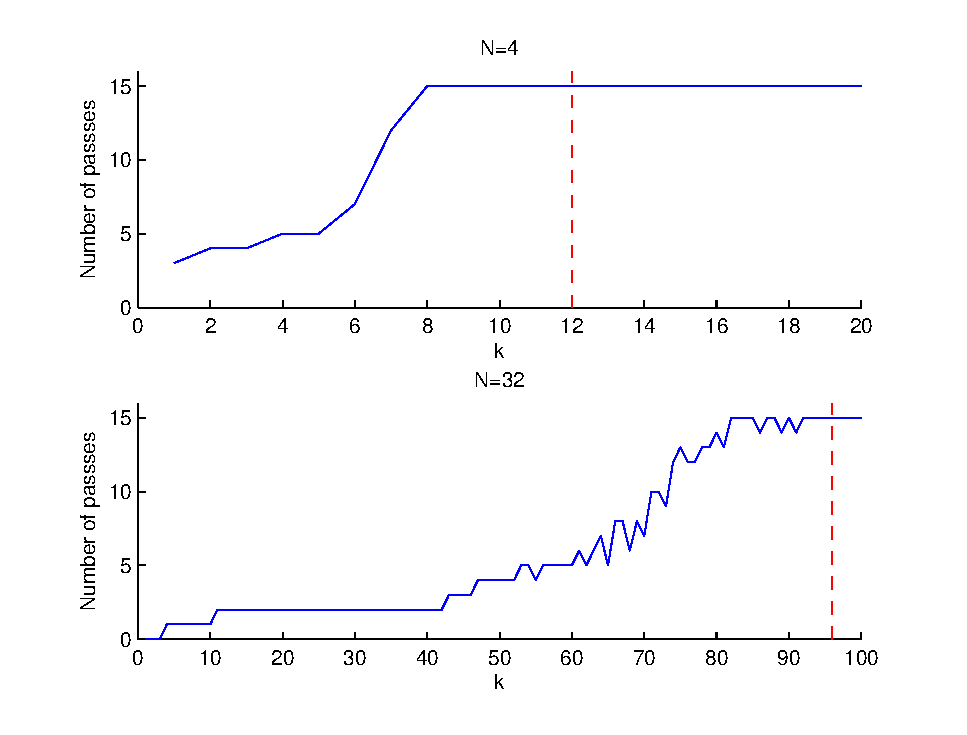
\includegraphics[scale=0.55]{images/correlation_c_sc.eps} 
\DeclareGraphicsExtensions.
\caption{Small Crush for CI(ISAAC,XORshift)}
\label{Small Crush for CI}
\end{figure}

\subsubsection{Correlation between TestU01 results and $\mathsf{N}$}

To compare the sequences generated with different parameters $\mathsf{N}$ in a more quantitative manner, we have set $k=3N+1$, and the same analysis for the four CI(X,Y) generators through TestU01 has been repeated. Let us recall that the TestU01 suite implements 518 tests and reports $p-$values, which must be within $[0.001,0.999]$ for a passing test.

\begin{figure*}
\centering
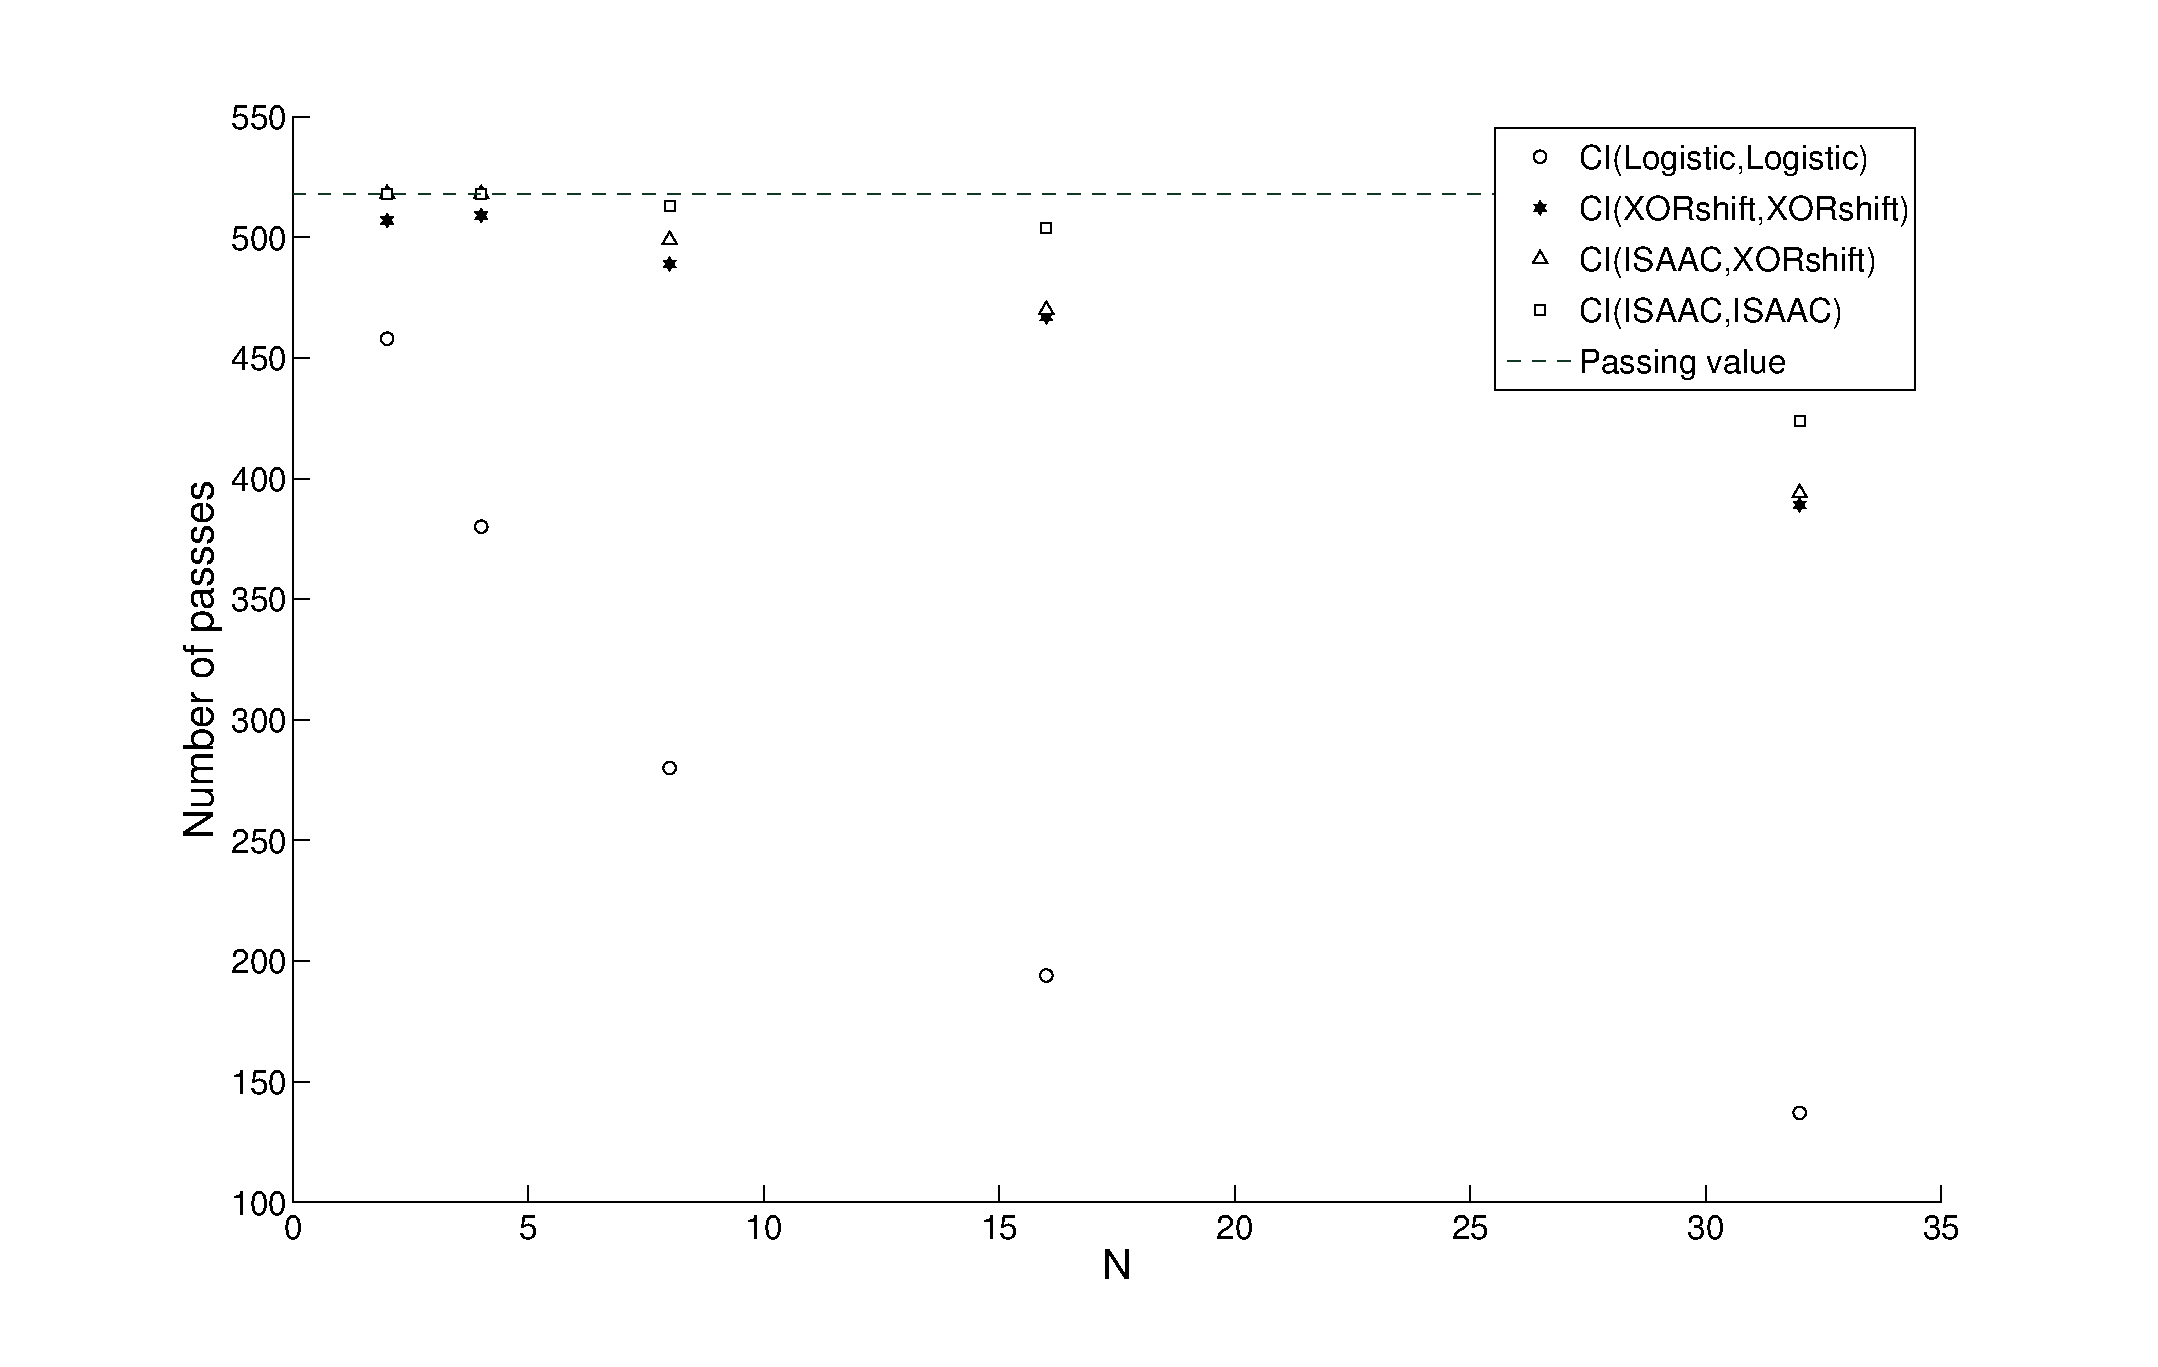
\includegraphics[scale=0.4]{images/N.eps} 
\DeclareGraphicsExtensions.
\caption{TestU01 results}
\label{TestU01 results}
\end{figure*}

Figure~\ref{TestU01 results} shows the number of passing sequences generated by the CI(X,Y) PRNGs proposed in this paper, with the same parameters and initial values. % (see the appendix for details).
It can be seen that $\mathsf{N}=4$ gives the best results.

For this reason, it is the default $\mathsf{N}=4$ with $k=12$ mode in following sections.
%As can be seen, the places where a sequence successfully passes most of the tests correspond nicely to the parameters for which $\mathsf{N}=4$.

\subsection{Results of NIST}

In our experiments, 100 sequences (s = 100) of 1,000,000 bits are generated and tested. If the value $\mathbb{P}_T$ of any test is smaller than 0.0001, the sequences are considered to not be good enough and the generator is unsuitable. Table~\ref{The passing for old CI} shows $\mathbb{P}_T$ of the sequences based on discrete chaotic iterations using different schemes. If there are at least two statistical values in a test, this test is marked with an asterisk and the average value is computed to characterize the statistical values. 


\begin{table}[!t]
\renewcommand{\arraystretch}{1.3}
\caption{NIST SP 800-22 test results ($\mathbb{P}_T$) for old CI algorithms ($\mathsf{N}=4$)}
\label{The passing for old CI}
\centering
  \begin{tabular}{lcccc}
    \toprule
\multirow{4}*{Test name} & \multicolumn{4}{c}{Old CI}\\
&Logistic& XORshift& ISAAC&ISAAC  \\ 
&+& +& + & + \\ 
&Logistic& XORshift& XORshift&ISAAC  \\ \cmidrule(r){2-5}
Frequency (Monobit) Test 			&0.85138	&0.59554	&0.40119		&0.33453 \\ 
Frequency Test within a Block  			&0.38382	&0.55442	&0.89776		&0.71974  \\ 
Runs Test 					&0.31908	&0.45593	&0.31908		&0.38382  \\ 
Longest Run of Ones in a Block Test 		&0.13728	&0.01671	&0.08558		&0.67868   \\
Binary Matrix Rank Test 			&0.69931	&0.61630	&0.47498		&0.79813  \\ 
Discrete Fourier Transform (Spectral) Test	&0.12962	&0.00019	&0.77918		&0.67868   \\ 
Non-overlapping Template Matching Test* 	&0.48473	&0.53225	&0.53568		&0.51258 \\ 
Overlapping Template Matching Test   		&0.47498	&0.33453	&0.36691		&0.07571  \\ 
Universal Statistical Test   			&0.09657	&0.03292	&0.26224		&0.85138   \\ 
Linear Complexity Test  			&0.41902	&0.40119	&0.61715		& 0.21330    \\ 
Serial Test* (m=10) 				&0.53427	&0.01339	&0.33453		&0.76102   \\ 
Approximate Entropy Test (m=10) 		&0.99146	&0.13728	&0.53414		&0.22482  \\ 
Cumulative Sums (Cusum) Test* 			&0.75530	&0.04646	&0.31915		& 0.47658\\ 
Random Excursions Test* 			&0.65406	&0.50362	&0.50804		&0.46305  \\ 
Random Excursions Variant Test* 		&0.55388	&0.34777	&0.48400		&0.54863    \\ \hline
Success 					&15/15		&15/15		&15/15		&15/15 \\ 
\bottomrule
  \end{tabular}
\end{table}


\subsection{Results of Diehard}
\label{Subsec:DieHARD}

Table~\ref{Results of DieHARD battery of tests for old CI algorithms} gives the results derived from applying the DieHARD battery of tests to the PRNGs considered in this work. 

\begin{tiny}
\begin{table}[!t]
\renewcommand{\arraystretch}{1.3}
\caption{Results of DieHARD battery of tests for old CI algorithms ($\mathsf{N}=4$)}
\label{Results of DieHARD battery of tests for old CI algorithms}
\centering
\begin{tabular}{llcccc} \toprule
\multirow{4}*{No.} &\multirow{4}*{Test name}& \multicolumn{4}{c}{Old CI}\\
&&Logistic& XORshift& ISAAC&ISAAC  \\ 
&&+& +& + & + \\ 
&&Logistic& XORshift& XORshift&ISAAC \\ \cmidrule(r){3-6}

1 & Overlapping Sum &Pass &Pass &Pass&Pass\\
2 & Runs Up 1 &Pass & Pass &Pass&Pass\\
&Runs Down 1 &Pass &Pass &Pass&Pass\\
&Runs Up 2 & Pass &Pass &Pass&Pass\\
&Runs Down 2 &Pass & Pass &Pass&Pass\\
3 & 3D Spheres &Pass &Pass &Pass&Pass\\
4 & Parking Lot &Pass &Pass &Pass&Pass\\
5 & Birthday Spacing &Pass &Pass &Pass&Pass\\
6 & Count the ones 1 &Pass &Pass &Pass&Pass\\
7 &Binary Rank $6 \times 8$ &Pass & Pass &Pass&Pass\\
8 &Binary Rank $31 \times 31$ &Pass &Pass &Pass&Pass\\
9 &Binary Rank $32 \times 32$ &Pass &Pass &Pass&Pass\\
10 &Count the ones 2 &Pass &Pass&Pass&Pass \\
11 &Bit Stream &Pass &Pass&Pass&Pass \\
12 &Craps Wins &Pass &Pass&Pass&Pass \\
&Throws &Pass &Pass &Pass&Pass\\
13 &Minimum Distance &Pass &Pass &Pass&Pass\\
14 &Overlapping Perm. &Pass &Pass &Pass&Pass\\
15 &Squeeze &Pass &Pass&Pass&Pass \\
16 &OPSO &Pass &Pass&Pass&Pass \\
17 &OQSO &Pass &Pass&Pass&Pass \\
18 &DNA &Pass &Pass&Pass &Pass\\
&Number of tests passed &18 &18 &18&18\\\bottomrule
\end{tabular}
\end{table}
\end{tiny}

\subsection{Results of comparative test parameters}

\begin{table}[!t]
\renewcommand{\arraystretch}{1.3}
\caption{Comparative test parameters for Old CI(X,Y) with a $10^7$ bits sequence ($\mathsf{N}=4$)}
\label{Comparison2 for old CI algorithms}
\centering
  \begin{tabular}{lccccc}
    \toprule
\multirow{4}*{Method} &\multirow{4}*{Threshold values} 	& \multicolumn{4}{c}{Old CI}\\
&&Logistic& XORshift& ISAAC&ISAAC  \\ 
&&+& +& + & + \\ 
&&Logistic& XORshift& XORshift&ISAAC \\ \cmidrule(r){3-6}
Monobit			&3.8415		&1.0368		&3.5689		&0.0569		&0.6641 \\ \hline
Serial  		&5.9915		&1.1758		&3.5765		&0.9828		&0.6506  \\ \hline
Poker  			&316.9194	&269.0607	&222.3683	&243.8415	&262.6440  \\ \hline
Runs 			&55.0027	&36.5479	&28.4237	&29.3195	&30.3116   \\ \hline
Autocorrelation		&1.6449		&0.4054		&0.3403		&0.6141		&0.9455  \\ \bottomrule
  \end{tabular}
\end{table}


We show in Table~\ref{Comparison2 for old CI algorithms} a comparison between old CI(Logistic, Logistic), old CI(XORshift, XORshift), old CI(ISAAC, XORshift), and old CI(ISAAC, ISAAC). %The comparative test is related to the duration needed by each algorithm to generate a $10^7$ bits long sequence. 


\subsection{Results of TestU01}
In a sound theoretical basis, a PRNG based on discrete chaotic iterations (CI) is a composite generator which combines the features of two PRNGs. The first generator constitutes the initial condition of the chaotic dynamical system. The second generator randomly chooses which outputs of the chaotic system must be returned. The intention of this combination is to cumulate the effects of chaotic and random behaviors, to improve the statistical and security properties relative to each generator taken alone.

This PRNG based on discrete chaotic iterations may utilize any reasonable RNG as inputs. For demonstration purposes, Logistic map, XORshift and ISAAC are adopted here. 

Table~\ref{TestU01 for old CI} gives the results derived from applying the TestU01 battery of tests to the PRNGs considered in this work.
\begin{table}[!t]
\renewcommand{\arraystretch}{1.3}
\caption{TestU01 Statistical Test for old CI algorithms ($\mathsf{N}=4$)}
\label{TestU01 for old CI}
\centering
  \begin{tabular}{lcccccc}
    \toprule
\multirow{4}*{Test name} &&& \multicolumn{4}{c}{Old CI}\\
&&&Logistic& XORshift& ISAAC&ISAAC  \\ 
&&&+& +& + & + \\ 
&&&Logistic& XORshift& XORshift&ISAAC  \\ \cmidrule(r){4-7}
Rabbit 				&$32\times10^9$ bits  	&38  	&7 	&2 	&0 	&0	 \\
Alphabit 			&$32\times10^9$ bits	&17 	& 3	&0 	&0 	&0	 \\
Pseudo DieHARD 			&Standard		&126 	&0 	&0 	&0 	&0	\\
FIPS\_140\_2 			&Standard		&16 	&0 	&0	&0 	&0	\\
Small Crush 			&Standard		&15 	&2 	&0	&0 	&0	 \\
Crush 				&Standard		&144 	&47 	&4 	&0 	&0	 \\
Big Crush 			&Standard		&160 	&79 	&3 	&0	&0	 \\ \hline
Number of failures 		& 			&518 	&138 	&9 	&0 	&0	 \\
\bottomrule
  \end{tabular}
\end{table}


\subsection{Conclusion}


Our old CI PRNG based on discrete chaotic iterations combines the features of two PRNGs, in order to improve their statistical properties. Logistic map, XORshift, and ISAAC are adopted here for demonstration purposes. 
The results of comparative test parameters confirm that the proposed CI PRNGs are all able to pass these tests.
Statistical results of comparative test parameters for both CI(XORshift, XORshift) and CI(ISAAC, XORshift) are better for most of the parameters, leading to the conclusion that these generators are more secure than the others. 
This improvement clearly appears in the TestU01 results: i.e. XORshift alone fails 142 of these tests, whereas  CI(XORshift, XORshift) only fails 9 out of 518.
In other words, in addition of having chaotic properties, our PRNG based on discrete chaotic iterations can pass more performed tests than its individual components taken alone. 


\section{Test results and comparative analysis for new CI}

\subsection{Results of NIST}
\label{Results of NISTfor new CI}
In our experiments, 100 sequences (s = 100) of 1,000,000 bits are generated and tested. If the value $\mathbb{P}_T$ of any test is smaller than 0.0001, the sequences are considered to not be good enough and the generator is unsuitable. Table~\ref{The passing rate1} and Table~\ref{The passing for new CI} show $\mathbb{P}_T$ of the sequences based on discrete chaotic iterations using different schemes. If there are at least two statistical values in a test, this test is marked with an asterisk and the average value is computed to characterize the statistical values. 

\begin{table}[!t]
\renewcommand{\arraystretch}{1.3}
\caption{SP 800-22 test results ($\mathbb{P}_T$) for new CI(XORshift, XORshift)  $\mathsf{N}=32$}
\label{The passing rate1}
\centering
\begin{tabular}{lcccc}
    \toprule
\multirow{2}*{Method} & \multicolumn{3}{c}{New CI}\\
 & $m^n=y^n~mod~N$&no mark&$g_2()$\\ \cmidrule(r){2-4}
%$w^{j}$ & $\{1,..,8\}$ & $\{1,..,8\}$ & $\{1,..,8\}$ & $\{1,..,5\}$ & $\{1,..,5\}$ &$\{1,..,5\}$ \\ \hline \hline
Frequency (Monobit) Test 			&0.00040	&0.08556		&0.41943\\ 
Frequency Test within a Block  			&0		&0			&0.67862\\ 
Runs Test  					&0.28966	&0.55448		&0.33452\\ 
Longest Run of Ones in a Block Test 		&0.01096	&0.43723		&0.88313 \\ 
Binary Matrix Rank Test  			&0		&0.65794		&0.75972\\ 
Discrete Fourier Transform (Spectral) Test 	&0		&0			&0.00085 \\ 
Non-overlapping Template Matching Test* 	&0.02007	&0.37333		&0.51879\\ 
Overlapping Template Matching Test		&0		&0	 	 	&0.24924\\ 
Maurer's ``Universal Statistical'' Test  	&0.69936	&0.96424		&0.12963\\ 
Linear Complexity Test 				&0.36699	&0.92423	 	&0.35045\\ 
Serial Test* (m=10) 				&0		&0.28185	 	&0.25496\\ 
Approximate Entropy Test (m=10) 		&0		&0.38381	 	&0.75971\\ 
Cumulative Sums (Cusum) Test* 			&0		&0			&0.34245\\ 
Random Excursions Test* 			&0.46769	&0.34788	 	&0.18977\\ 
Random Excursions Variant Test* 		&0.28779	&0.46505		&0.26563\\ \hline
Success 					&8/15		&11/15		  	&15/15\\ 
\bottomrule
\end{tabular}
\end{table}

We can conclude from Table \ref{The passing rate1} that the worst situations are obtained with the New CI ($m^n=y^n~mod~N$) and New CI (no mark) generators. %: they just can be observed that 8 and 11 out of 15 of the tests are failed. However,
New CI ($m^n=g_2(y^n)$) as New CI ($m^n=g_1(y^n)$) in Table~\ref{The passing for new CI} has successfully passed the NIST statistical test suite.

\begin{table}[!t]
\renewcommand{\arraystretch}{1.3}
\caption{NIST SP 800-22 test results ($\mathbb{P}_T$) for new CI algorithms}
\label{The passing for new CI}
\centering
  \begin{tabular}{lccc}
    \toprule
\multirow{4}*{Test name} & \multicolumn{3}{c}{New CI}\\
& XORshift& ISAAC&ISAAC  \\ 
& +& + & + \\ 
& XORshift& XORshift&ISAAC  \\  \cmidrule(r){2-4}
Frequency (Monobit) Test 			&0.47498 		&0.88317		&0.83430 \\ 
Frequency Test within a Block  			&0.89776		&0.40119		&0.33453  \\ 
Runs Test 					&0.81653		&0.31908		&0.00576  \\ 
Longest Run of Ones in a Block Test 		&0.79813		&0.06688		&0.47498   \\
Binary Matrix Rank Test 			&0.26224		&0.88317		&0.69931  \\ 
Discrete Fourier Transform (Spectral) Test	&0.00716		&0.33453		&0.59559   \\ 
Non-overlapping Template Matching Test* 	&0.44991		&0.46467		&0.51446 \\ 
Overlapping Template Matching Test   		&0.51412		&0.69931		&0.88317  \\ 
Universal Statistical Test   			&0.67868		&0.24928		&0.06282   \\ 
Linear Complexity Test  			&0.65793		&0.65793		&0.94630     \\ 
Serial Test* (m=10) 				&0.42534		&0.90619		&0.44137   \\ 
Approximate Entropy Test (m=10) 		&0.63719		&0.22482		&0.13728  \\ 
Cumulative Sums (Cusum) Test* 			&0.27968		&0.84065		&0.14139 \\ 
Random Excursions Test* 			&0.28740		&0.30075		&0.34625   \\ 
Random Excursions Variant Test* 		&0.48668		&0.34294		&0.55048    \\ \hline
Success 					& 15/15			&15/15		&15/15	 \\ 
\bottomrule
  \end{tabular}
\end{table}

\subsection{Results of Diehard}
\label{Subsec:DieHARD}

Table~\ref{Results of DieHARD battery of tests for new CI algorithms} gives the results derived from applying the DieHARD battery of tests to the PRNGs considered in this work. 

\begin{tiny}
\begin{table}[!t]
\renewcommand{\arraystretch}{1.3}
\caption{Results of DieHARD battery of tests for new CI algorithms ($\mathsf{N}=32$)}
\label{Results of DieHARD battery of tests for new CI algorithms}
\centering
\begin{tabular}{llcccc} \toprule
\multirow{3}*{No.} &\multirow{3}*{Test name} & \multicolumn{4}{c}{New CI}\\
&&Logistic& XORshift& ISAAC&ISAAC  \\ 
&&+& +& + & + \\ 
&&Logistic& XORshift& XORshift&ISAAC \\ \cmidrule(r){3-6}
1 & Overlapping Sum &Pass &Pass &Pass&Pass\\
2 & Runs Up 1 &Pass & Pass &Pass&Pass\\
&Runs Down 1 &Pass &Pass &Pass&Pass\\
&Runs Up 2 & Pass &Pass &Pass&Pass\\
&Runs Down 2 &Pass & Pass &Pass&Pass\\
3 & 3D Spheres &Pass &Pass &Pass&Pass\\
4 & Parking Lot &Pass &Pass &Pass&Pass\\
5 & Birthday Spacing &Pass &Pass &Pass&Pass\\
6 & Count the ones 1 &Pass &Pass &Pass&Pass\\
7 &Binary Rank $6 \times 8$ &Pass & Pass &Pass&Pass\\
8 &Binary Rank $31 \times 31$ &Pass &Pass &Pass&Pass\\
9 &Binary Rank $32 \times 32$ &Pass &Pass &Pass&Pass\\
10 &Count the ones 2 &Pass &Pass&Pass&Pass \\
11 &Bit Stream &Pass &Pass&Pass&Pass \\
12 &Craps Wins &Pass &Pass&Pass&Pass \\
&Throws &Pass &Pass &Pass&Pass\\
13 &Minimum Distance &Pass &Pass &Pass&Pass\\
14 &Overlapping Perm. &Pass &Pass &Pass&Pass\\
15 &Squeeze &Pass &Pass&Pass&Pass \\
16 &OPSO &Pass &Pass&Pass&Pass \\
17 &OQSO &Pass &Pass&Pass&Pass \\
18 &DNA &Pass &Pass&Pass &Pass\\
&Number of tests passed &18 &18 &18&18\\\bottomrule
\end{tabular}
\end{table}
\end{tiny}

\subsection{Results of comparative test parameters}



\begin{table}[!t]
\renewcommand{\arraystretch}{1.3}
\caption{Comparative test parameters for new CI(X,Y) with a $10^7$ bits sequence ($\mathsf{N}=32$)}
\label{Comparison2 for new CI algorithms}
\centering
  \begin{tabular}{lcccc}
    \toprule
\multirow{4}*{Method} &\multirow{4}*{Threshold values} 	& \multicolumn{3}{c}{New CI}\\
&& XORshift& ISAAC&ISAAC  \\ 
&& +& + & + \\ 
&& XORshift& XORshift&ISAAC \\ \cmidrule(r){2-5}
Monobit			&3.8415				&3.5689		&0.9036		&0.5788 \\ \hline
Serial  		&5.9915				&3.5765		&1.1229		&0.7378  \\ \hline
Poker  			&316.9194			&123.6831	&173.8604		&179.8609  \\ \hline
Runs 			&55.0027			&28.4237	&40.4606	&29.4057   \\ \hline
Autocorrelation		&1.6449				&0.3403		&0.1245		&-2.0276 \\ \bottomrule
  \end{tabular}
\end{table}

We show in Table~\ref{Comparison2 for new CI algorithms} a comparison between New CI(XORshift, XORshift), New CI(ISAAC, XORshift), and New CI(ISAAC, ISAAC). %The comparative test is related to the duration needed by each algorithm to generate a $10^7$ bits long sequence. 

\subsection{Results of TestU01}


Table~\ref{TestU01 for new CI} gives the results derived from applying the TestU01 battery of tests to the PRNGs considered in this work.
\begin{table}[!t]
\renewcommand{\arraystretch}{1.3}
\caption{TestU01 Statistical Test for new CI algorithms ($\mathsf{N}=32$)}
\label{TestU01 for new CI}
\centering
  \begin{tabular}{lccccc}
    \toprule
\multirow{4}*{Test name} &&& \multicolumn{3}{c}{New CI}\\
&&&Logistic& ISAAC&ISAAC  \\ 
&&&+& +& + \\ 
&&&Logistic& XORshift&ISAAC  \\ \cmidrule(r){4-6}
Rabbit 				&$32\times10^9$ bits  	&38  	&0 	&0 	&0 		 \\
Alphabit 			&$32\times10^9$ bits	&17 	&0 	&0 	&0 		 \\
Pseudo DieHARD 			&Standard		&126 	&0 	&0 	&0 		\\
FIPS\_140\_2 			&Standard		&16 	&0 	&0 	&0 		\\
Small Crush 			&Standard		&15 	&0	&0	&0 		 \\
Crush 				&Standard		&144 	&0 	&0 	&0 		 \\
Big Crush 			&Standard		&160 	&0 	&0 	&0		 \\ \hline
Number of failures 		& 			& 	&0 	&0	&0 		 \\
\bottomrule
  \end{tabular}
\end{table}


\subsection{Conclusion}
In a sound theoretical basis, a New PRNG based on discrete chaotic iterations (CI) is a composite generator which combines the features of two PRNGs. The first generator constitutes the initial condition of the chaotic dynamical system. The second generator randomly chooses which outputs of the chaotic system must be returned. The intention of this combination is to cumulate the effects of chaotic and random behaviors, to improve the statistical and security properties relative to each generator taken alone.

This New CI PRNG based on discrete chaotic iterations may utilize any reasonable RNG as inputs. For demonstration purposes, XORshift and ISAAC are adopted here. 

The results of the TestU01, NIST, Comparative test parameters and DieHARD batteries of tests confirm that the proposed New CI PRNGs are all able to pass these tests. And it is better than Old CI algorithms

The improvement clearly appears in the TestU01 results: i.e. XORshift alone fails 142 of these tests, whereas  Old CI(XORshift, XORshift) fails 9 out of 518, New CI(XORshift, XORshift) can pass all the tests. 

Detail comparative analysis will be presented in the next section.


\section{Assessment of two chaotic iterations schemes based on XORshift Generator}

\subsection{NIST}

In our experiments, 100 sequences (s = 100) of 1,000,000 bits are generated and tested. If the value $\mathbb{P}_T$ of any test is smaller than 0.0001, the sequences are considered to not be good enough and the generator is unsuitable. Table~\ref{The passing} shows $\mathbb{P}_T$ of the sequences based on discrete chaotic iterations using different schemes. If there are at least two statistical values in a test, this test is marked with an asterisk and the average value is computed to characterize the statistical values. 
We can conclude from Table \ref{The passing} that XORshift has failed 1 test, whereas both the old generator and CI(XORshift, XORshift) have successfully passed the NIST statistical test suite. This result shows the good behavior of both PRNGs in the aforementioned basic tests that evaluate the independence of real numbers.

\begin{table}[!t]
\renewcommand{\arraystretch}{1.3}
\caption{NIST SP 800-22 test results ($\mathsf{N}=32$)}
\label{The passing}
\centering
  \begin{tabular}{|l||c|c|c|}
    \hline
Method &XORshift& Old CI & New CI  \\ \hline\hline

Frequency (Monobit) Test 			&0.145326&0.595549&0.474986 \\ \hline
Frequency Test within a Block  			&0.455937&0.554420&0.897763  \\ \hline
Runs Test 					&0.213309&0.455937&0.816537 \\ \hline
Longest Run of Ones in a Block Test 		&0.289667&0.016717&0.798139   \\ \hline
Binary Matrix Rank Test 			&0.000000&0.616305&0.262249  \\ \hline
Discrete Fourier Transform (Spectral) Test	&0.005358&0.000190&0.007160   \\ \hline
Non-overlapping Template Matching Test* 	&0.503652&0.532252&0.449916 \\ \hline
Overlapping Template Matching Test   		&0.867692&0.334538&0.514124  \\ \hline
Universal Statistical Test   			&0.275709&0.032923&0.678686  \\ \hline
Linear Complexity Test  			&0.924076&0.401199&0.657933    \\ \hline
Serial Test* (m=10) 				&0.757925&0.013396&0.425346  \\ \hline
Approximate Entropy Test (m=10) 		&0.419021&0.137282&0.637119  \\ \hline
Cumulative Sums (Cusum) Test* 			&0.8115445&0.046464&0.279680\\ \hline
Random Excursions Test* 			&0.4192395&0.503622&0.287409   \\ \hline
Random Excursions Variant Test* 		&0.5283333&0.347772&0.486686    \\ \hline
Success 					& 14/15	  & 15/15  & 15/15 \\ \hline

  \end{tabular}
\end{table}

\subsection{Diehard}
\label{Subsec:DieHARD}

Table~\ref{Results of DieHARD battery of tests} gives the results derived from applying the DieHARD battery of tests to the PRNGs considered in this work. As it can be observed, the results of the individual tests Count the ones 1, Binary Rank $31 \times 31$ and Binary Rank $32 \times 32$ show that in the random numbers obtained with the XORshift generator only the least significant bits seem to be independent. This explains the poor behavior of this PRNG in the aforementioned basic tests that evaluate the independence of real numbers. But the generator based on discrete chaotic iterations (New CI and Old CI PRNG) can pass all the DieHARD battery of tests. 
This proves that the
security of the given generator has been improved by chaotic iterations.

\begin{tiny}
\begin{table}[!t]
\renewcommand{\arraystretch}{1.3}
\caption{Results of DieHARD battery of tests ($\mathsf{N}=32$)}
\label{Results of DieHARD battery of tests}
\centering
\begin{tabular}{llccc} \toprule
\textbf{No.} &\textbf{Test name} &\multicolumn{3}{c}{\textbf{Generators}} \\ \cmidrule(r){3-5}
& & XORshift &  Old CI & New CI\\ \midrule
1 & Overlapping Sum &Pass &Pass &Pass\\
2 & Runs Up 1 &Pass & Pass &Pass\\
&Runs Down 1 &Pass &Pass &Pass\\
&Runs Up 2 & Pass &Pass &Pass\\
&Runs Down 2 &Pass & Pass &Pass\\
3 & 3D Spheres &Pass &Pass &Pass\\
4 & Parking Lot &Pass &Pass &Pass\\
5 & Birthday Spacing &Pass &Pass &Pass\\
6 & Count the ones 1 &Fail &Pass &Pass\\
7 &Binary Rank $6 \times 8$ &Pass & Pass &Pass\\
8 &Binary Rank $31 \times 31$ &Fail &Pass &Pass\\
9 &Binary Rank $32 \times 32$ &Fail &Pass &Pass\\
10 &Count the ones 2 &Pass &Pass&Pass \\
11 &Bit Stream &Pass &Pass&Pass \\
12 &Craps Wins &Pass &Pass&Pass \\
&Throws &Pass &Pass &Pass\\
13 &Minimum Distance &Pass &Pass &Pass\\
14 &Overlapping Perm. &Pass &Pass &Pass\\
15 &Squeeze &Pass &Pass&Pass \\
16 &OPSO &Pass &Pass&Pass \\
17 &OQSO &Pass &Pass&Pass \\
18 &DNA &Pass &Pass&Pass \\
&Number of tests passed &15 &18 &18\\\bottomrule
\end{tabular}
\end{table}
\end{tiny}

\subsection{Comparative test parameters}

\begin{table}
\renewcommand{\arraystretch}{1.3}
\caption{Comparison with Old CI(XORshift,XORshift) for a $2 \times 10^5$ bits sequence  ($\mathsf{N}=32$)}
\label{Comparison22}
\centering
  \begin{tabular}{lcccc}
    \toprule
Method &The threshold values&XORshift& Old CI& New CI \\ \hline
   
Monobit			&3.8415		&1.7053		&2.7689		&0.3328	 \\ \hline
Serial  		&5.9915		&2.1466		&2.8765		&0.7441		  \\ \hline
Poker  			&316.9194	&248.9318	&222.3683	&262.8173		 \\ \hline
Runs 			&55.0027	&18.0087	&21.9272	&16.7877	   \\ \hline
Autocorrelation		&1.6449		&0.5009		&0.0173		&0.0805		  \\ \hline
Time			&Second		&0.096s		&0.3625s	&0.197s		  \\ 
    \bottomrule
  \end{tabular}
\end{table}



We show in Table~\ref{Comparison22} a comparison between our new generator New CI(XORshift, XORshift), its old version denoted Old CI(XORshift, XORshift), and a PRNG based on a simple XORshift. Time (in seconds) is related to the duration needed by each algorithm to generate a $2 \times 10^5$ bits long sequence. The test has been conducted using the same computer and compiler with the same optimization settings for both algorithms, in order to make it as fair as possible. 
The results confirm that the proposed generator is a lot faster than the old one, while the statistical results are better for most of the parameters, leading to the conclusion that the new PRNG is more secure than the old one. % The main advantage of our new method lies in its flexibility, therefore optimizing for higher speeds, better security or low memory requirements.


\begin{figure}
\centering
% \psfig{figure=2.eps,height=5in,width=3.5in}
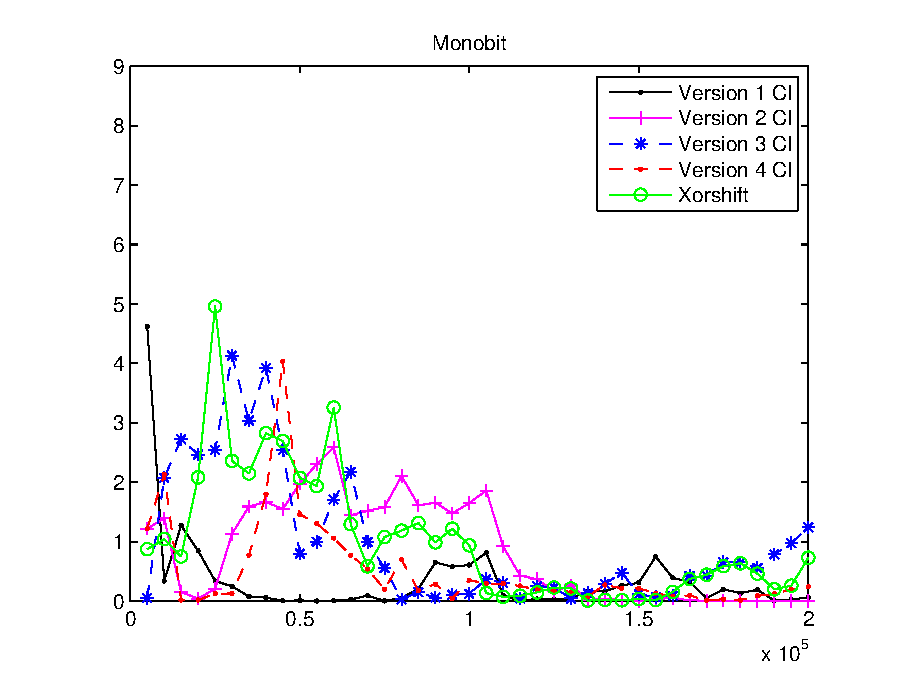
\includegraphics[scale=0.4]{monobits.eps}
% \includegraphics[width=3.7in]{4tests.eps}
\caption{Comparison of monobits tests}
\label{monobits}
\end{figure}

As a comparison of the overall stability of these PRNGs, similar tests have been computed for different sequence lengths (see Figures \ref{monobits} - \ref{autocorrelation}).
For the monobit test comparison (Figure \ref{monobits}), XORshift and New CI(XORshift, XORshift) PRNGs present the same issue: the beginning values are a little high. However, for our new generator, the values are stable in a low level which never exceeds 1.2. Indeed, the new generator distributes very randomly the zeros and ones, whatever the length of the desired sequence. 
It can also be remarked that the old generator presents the worst performance, but the values are  still within the standard boundary.
% The main advantage of our new method lies in its flexibility, therefore optimizing for higher speeds, better security or low memory requirements.

\begin{figure}
\centering
% \psfig{figure=2.eps,height=5in,width=3.5in}
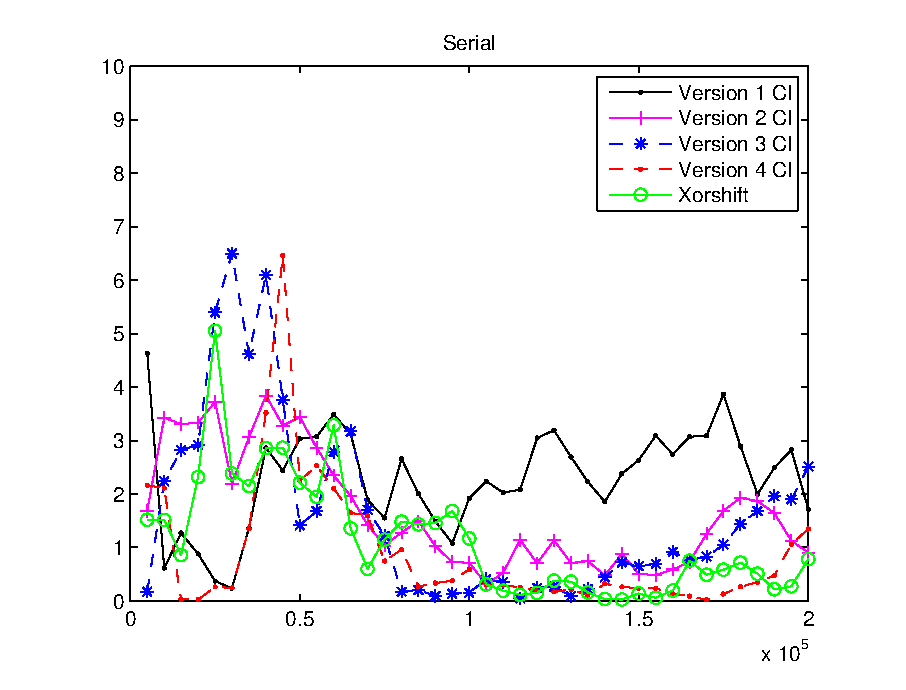
\includegraphics[scale=0.4]{serial.eps}
% \includegraphics[width=3.7in]{4tests.eps}
\caption{Comparison of serial tests}
\label{serial}
\end{figure}

Figure \ref{serial} shows the serial test comparison. The new generator outperforms this test, but the score of the old generator is not bad either: their occurrences of 00, 01, 10, and 11 are very close to each other.% As the same with monobit test, this phenomenon is attributed to the effect of iteration computation.

\begin{figure}
\centering
% \psfig{figure=2.eps,height=5in,width=3.5in}
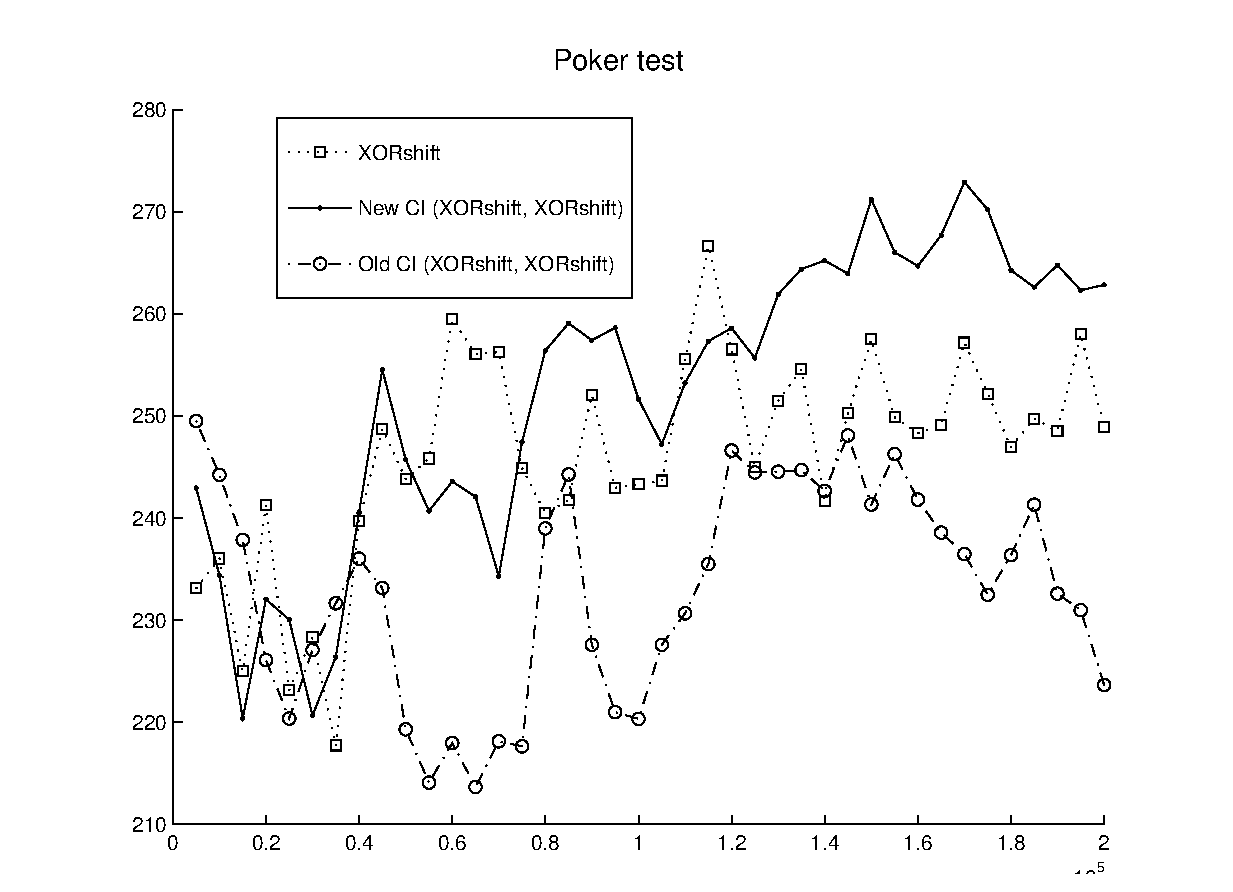
\includegraphics[scale=0.4]{poker.eps}
% \includegraphics[width=3.7in]{4tests.eps}
\caption{Comparison of poker tests}
\label{poker}
\end{figure}

The poker test comparison with $m=8$ is shown in Figure \ref{poker}. XORshift is the most stable generator in all of these tests, but not better than Old CI(XORshift, XORshift) PRNG. 
Our new generator presents a trend, with a maximum in the neighborhood of $1.7 \times 10^5$. These scores are not so good, even though the new generator has a better behavior than the old one and XORshift. 
%The reasons explaining this bad result can be, among other:
Indeed, the value of $m$ and the length of the sequences should be enlarged to be certain that the chaotic iterations express totally their complex behavior. In that situation, the performances of our generators in the poker test can be improved.
%but here we only achieve $2 \times 10^5$ sequence length, then m must be smaller than 13 to comply with the rule, if the sequence length is more, the performance of CI might be better.

\begin{figure}
\centering
% \psfig{figure=2.eps,height=5in,width=3.5in}
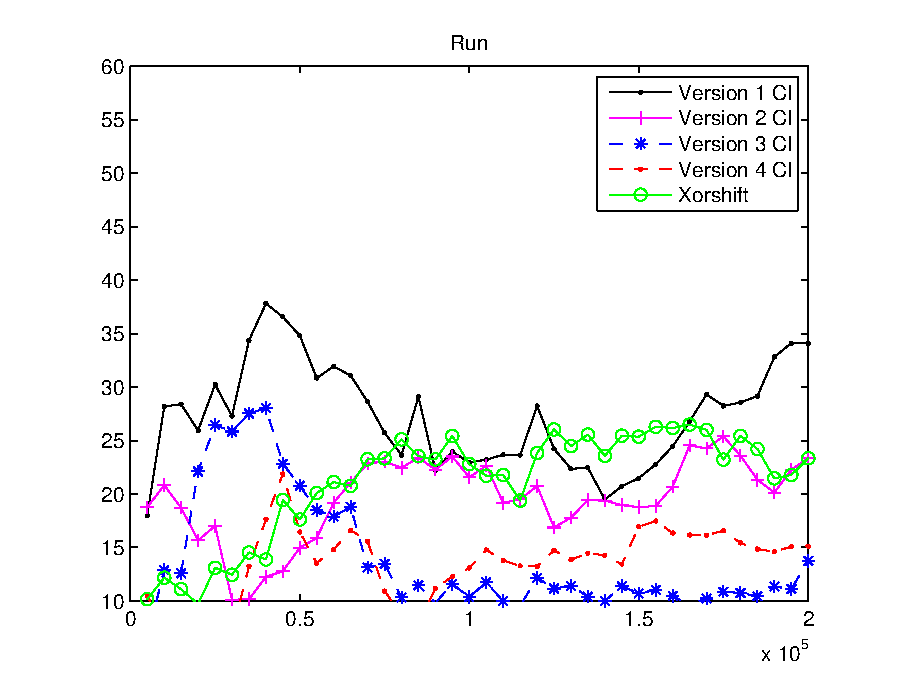
\includegraphics[scale=0.4]{runs.eps}
% \includegraphics[width=3.7in]{4tests.eps}
\caption{Comparison of runs tests}
\label{runs}
\end{figure}

The graph of the new generator is the most stable one during the runs test comparison (Figure \ref{runs}). Moreover, this trend is reinforced when the lengths of the tested sequences are increased.


\begin{figure}
\centering
% \psfig{figure=2.eps,height=5in,width=3.5in}
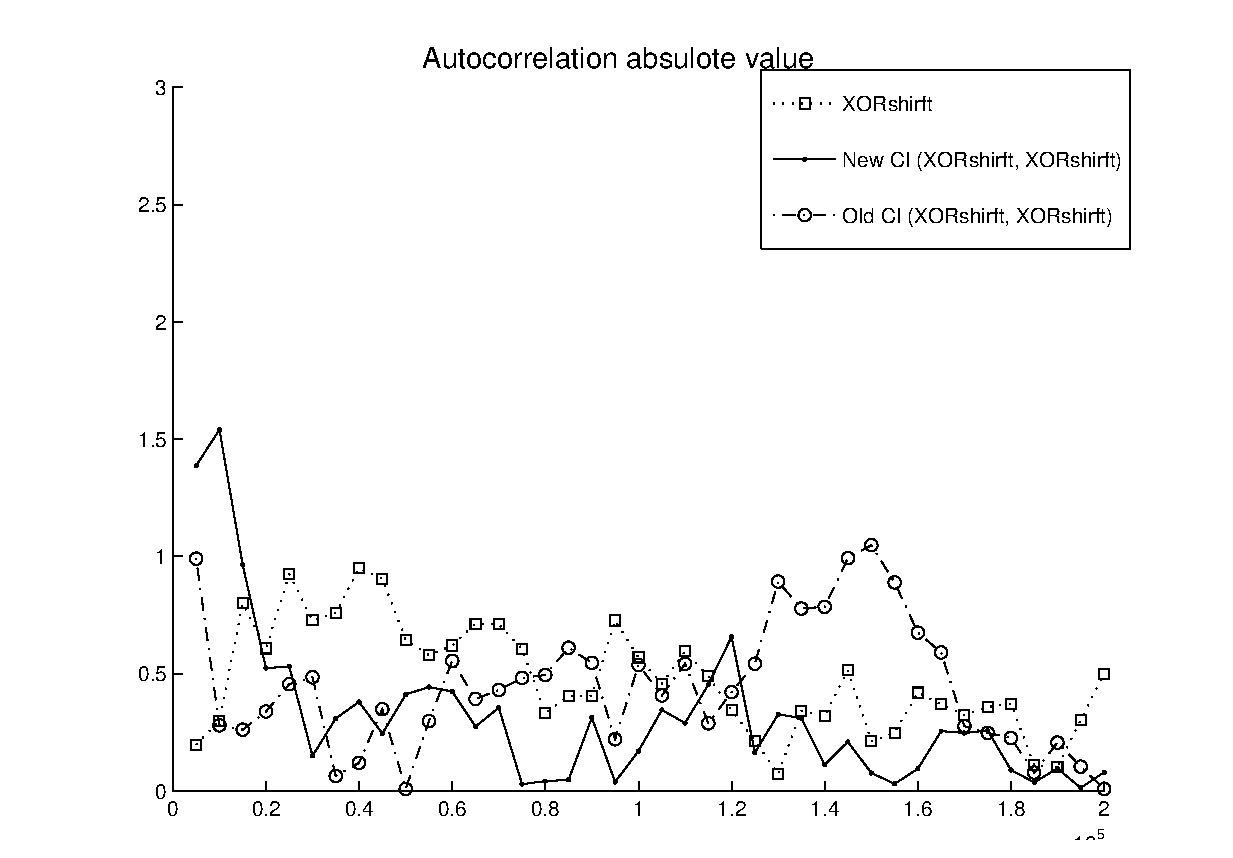
\includegraphics[scale=0.4]{autocorrelation1.eps}
% \includegraphics[width=3.7in]{4tests.eps}
\caption{Comparison of autocorrelation tests}
\label{autocorrelation}
\end{figure}


The comparison of autocorrelation tests is presented in Figure \ref{autocorrelation}. The new generator clearly dominates these tests, whereas the score of the old generator is also not bad. This difference between two generators based on chaotic iterations can be explained by the fact that the improvements realized to define the new generator lead to a more randomly output.

To sum up we can claim that the new generator, which is faster than its former version, outperforms all of the other generators in these statistical tests, especially when producing long output sequences.




\subsection{A flexible output}

We assume that the initial state $X$ is given as arrays of N-bit integers. Thus, the output size can be flexibly chosen  as well as $N$. Our PRNGs can generate discrete numbers
where the number of states could not match to a power of 2, which is suitable for stochastic differential equations as an example.(An attractive property of discrete random numbers is that they
require a small number of random bits--3 bits)~\cite{Ladd20092140}.
Moreover, due to the fact that CI process is a simple bitwise change, the speed of output integers and binary numbers is almost the same. 

In the following section, we will discuss the security level for various $N$ by Statistical test.
For both CI generator, various $N$ can pass all the NIST and DIEHARD test. Table~\ref{TestU01 Statistical Test} gives the results derived from applying the TestU01 battery of tests to the PRNGs considered in this work. As observed,  we can conclude that the effective range of $N$ for new CI is bigger than for old CI by TestU01. And also, this new scheme for obtaining a PRNG by combining two XORshift generators in CI give better properties than the old one (and the individual XORshift alone). It can be observed that the XORshift generator fails 146 tests.

\begin{table}[!t]
\begin{small}
\centering
\renewcommand{\arraystretch}{1.3}
\caption{TestU01 Statistical Test}
\label{TestU01 Statistical Test}
\centering
\begin{tabular}{cccccccccc}\toprule
\textbf{CI PRNG}&\textbf{Battery}&\textbf{N=2}&\textbf{N=4}&\textbf{N=8}&\textbf{N=16}&\textbf{N=32} \\\midrule

\multirow{7}*{\textbf{Old CI}}&Rabbit  					 	&2	&2	&2	&2	&3 \\
\multirow{7}*{\textbf{(XORshift,XORshift)}}&Alphabit 				&0	&0	&0	&2	&2 \\
&Pseudo DieHARD 								&0	&0	&0	&0	&0 \\
&FIPS\_140\_2 		 							&0	&0	&0	&0	&0 \\
&Small Crush 		 							&0	&0	&0	&1	&0 \\
&Crush 		 								&4	&4	&9	&16	&46 \\
&Big Crush 									&5	&3	&18	&30	&78 \\ 
\\
&Number of failures 	 							&11	&9	&29	&51	&129 \\
\bottomrule

\multirow{7}*{\textbf{New CI}}&Rabbit 					  	&0	&0	&0	&0	&0 \\
\multirow{7}*{\textbf{(XORshift,XORshift)}}&Alphabit 				&4	&0	&0	&0	&0 \\
&Pseudo DieHARD 	 							&8	&2	&0	&0	&0 \\
&FIPS\_140\_2		 							&2	&0	&0	&0	&0 \\
&Small Crush 		 							&0	&0	&0	&0	&0 \\
&Crush 										&0	&0	&0	&0	&0 \\
&Big Crush 		 							&0	&0	&0	&0	&0 \\ 
\\
&Number of failures 	 							&14	&2	&0	&0	&0 \\
\bottomrule
\end{tabular}
\end{small}
\end{table}

